% Chapter 2

\chapter{Navigation Among Movable Obstacles: state of the art} % Main chapter title

\label{Chapter2} % For referencing the chapter elsewhere, use \ref{Chapter2}

\section{Determining appropriate comparison criteria}

\subsection{Hypotheses}

\subsection{Approaches}

\subsection{Performance criteria}

\begin{figure}[H]
\centering
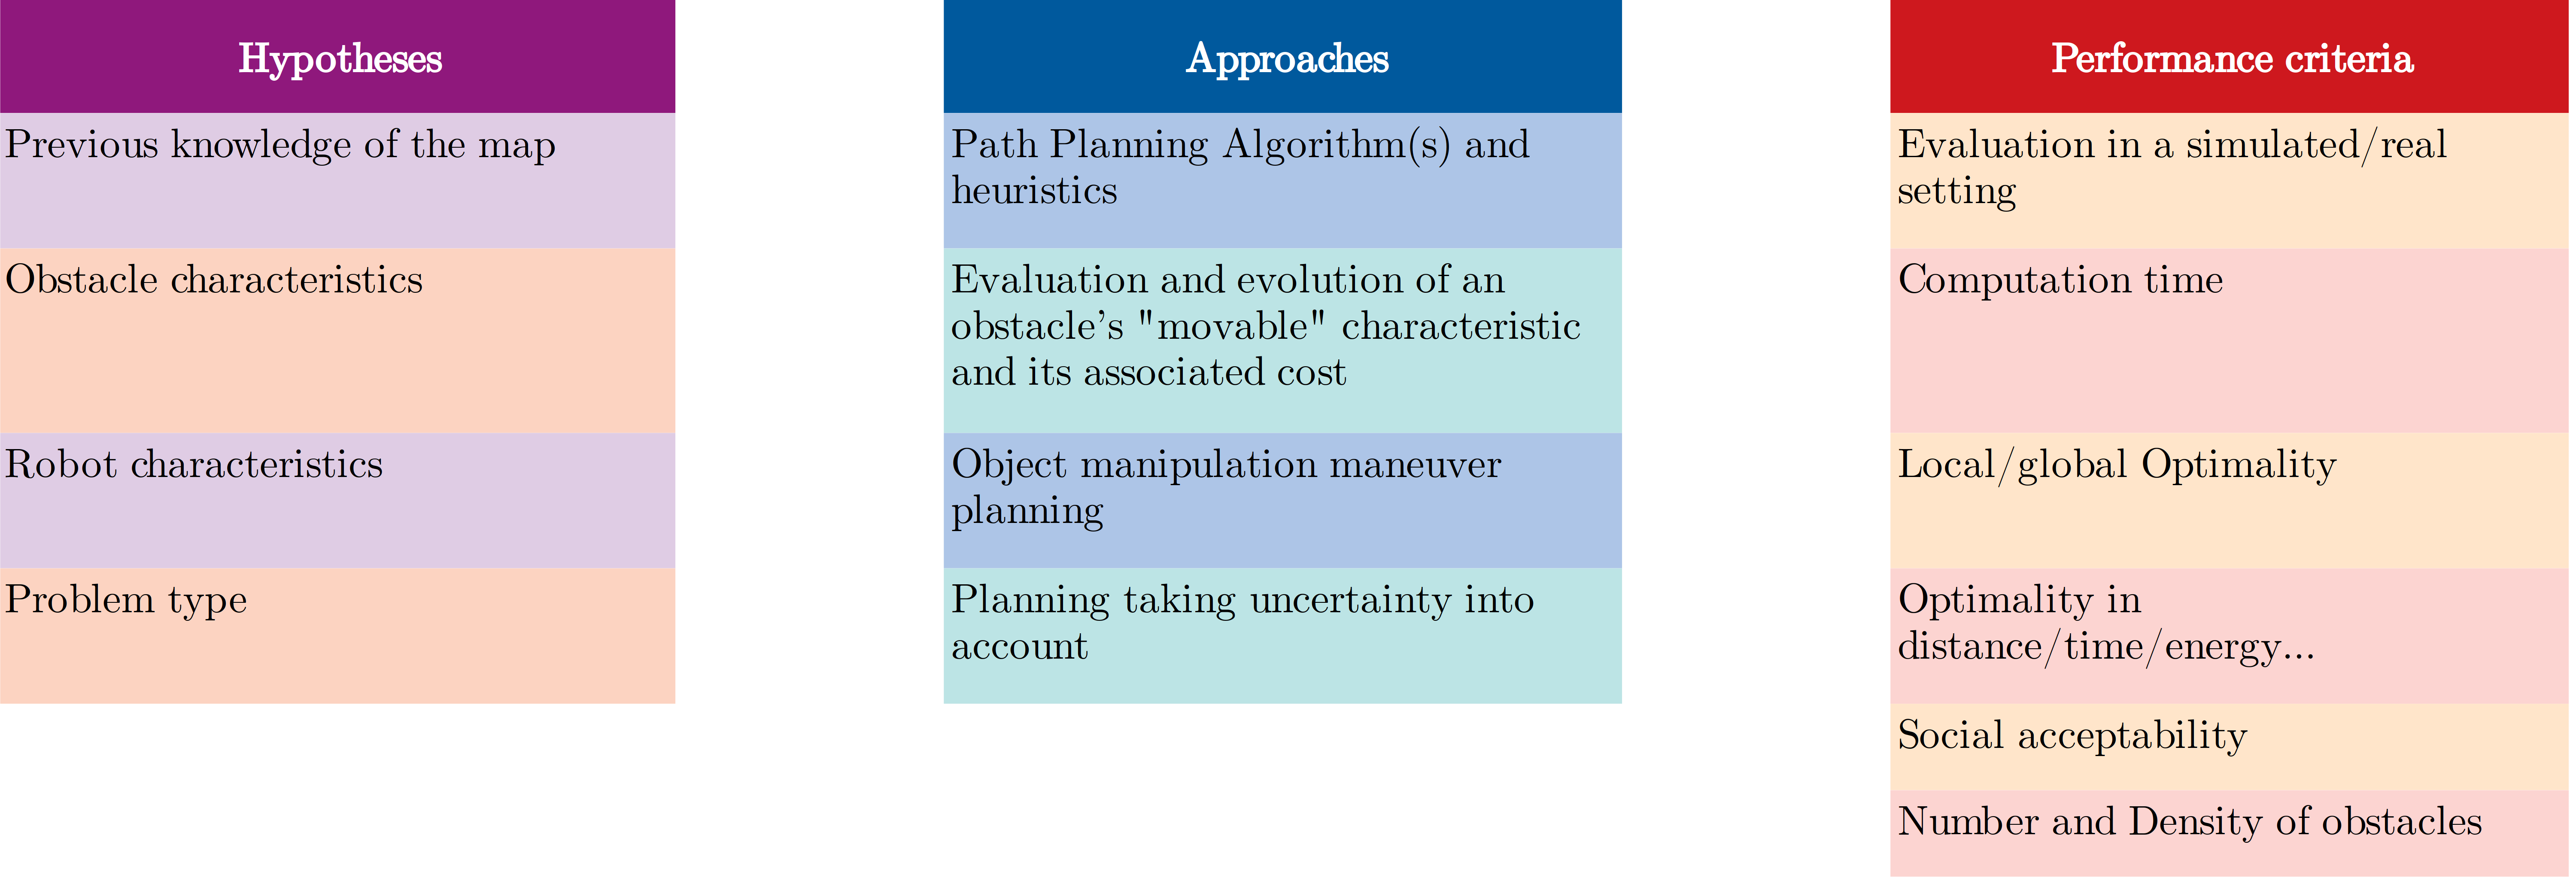
\includegraphics[width=13cm]{Comparison_Table/comparison_criteria}
\decoRule
\caption[Comparison criteria listing]{Comparison criteria, sorted by type: hypotheses, approaches and performance criterias}
\label{fig:comparison_criteria}
\end{figure}

\section{Comparison and cross-comparison}

\subsection{Comparison tables}

\subsection{Conclusions}

\subsection{Situating our work in the established context}
